% shared preamble of the theory figures (white background, purple / black theme, sans-serif)
\documentclass[tikz,border=8pt]{standalone}
\usepackage[T1]{fontenc}
\usepackage[scaled=0.92]{helvet}
\renewcommand{\familydefault}{\sfdefault}
\usepackage{amsmath,amssymb}
\usepackage[helvet]{sfmath}
\usetikzlibrary{arrows.meta,calc,decorations.pathreplacing,positioning,backgrounds}
\definecolor{ink}{HTML}{1A1A1F}
\definecolor{cohesin}{HTML}{6A3DE8}
\definecolor{condensin}{HTML}{1BAF7A}
\definecolor{fwd}{HTML}{D1303F}      % CTCF pointing right
\definecolor{rev}{HTML}{2B62D9}      % CTCF pointing left
\definecolor{panel}{HTML}{F8F6FD}
\definecolor{panelline}{HTML}{E3DDF5}
\tikzset{
  fiber/.style={line width=2.1pt,ink,line cap=round,line join=round},
  halo/.style={line width=6pt,white,line cap=round},
  lab/.style={font=\small,text=ink},
  note/.style={font=\footnotesize,text=ink!60},
  hd/.style={font=\bfseries\small,text=ink,anchor=west},
  leader/.style={line width=0.6pt,ink!45},
}
% soft panel, numbered badge, heading
\newcommand{\panelbg}[4]{\draw[rounded corners=9pt,fill=panel,draw=panelline,line width=0.9pt] (#1,#2) rectangle (#3,#4);}
\newcommand{\badge}[3]{\fill[ink] (#1,#2) circle (0.21);\node[white,font=\bfseries\footnotesize] at (#1,#2) {#3};}
% CTCF: a protein on the fibre carrying an arrow that gives the motif direction (f = right, r = left)
\newcommand{\protf}[2]{\draw[rounded corners=3.5pt,line width=0.6pt,draw=fwd!65!black,fill=fwd] (#1-0.3,#2-0.19) rectangle (#1+0.3,#2+0.19);
  \draw[white,line width=1.5pt,-{Stealth[length=3.4pt,width=4.4pt]}] (#1-0.15,#2)--(#1+0.16,#2);}
\newcommand{\protr}[2]{\draw[rounded corners=3.5pt,line width=0.6pt,draw=rev!65!black,fill=rev] (#1-0.3,#2-0.19) rectangle (#1+0.3,#2+0.19);
  \draw[white,line width=1.5pt,-{Stealth[length=3.4pt,width=4.4pt]}] (#1+0.15,#2)--(#1-0.16,#2);}
\newcommand{\prot}[3]{\csname prot#3\endcsname{#1}{#2}}
% ring seen at an angle, drawn as a tube (dark outline, light core); back half and front half
\newcommand{\ringpart}[5]{\draw[line width=4.6pt,#3!80!black,line cap=round] ([shift={(#1,#2)}]#4:0.55 and 0.21) arc[start angle=#4,end angle=#5,x radius=0.55,y radius=0.21];
  \draw[line width=2.4pt,#3!55!white,line cap=round] ([shift={(#1,#2)}]#4:0.55 and 0.21) arc[start angle=#4,end angle=#5,x radius=0.55,y radius=0.21];}
\newcommand{\ringback}[3]{\ringpart{#1}{#2}{#3}{180}{0}}
\newcommand{\ringfront}[3]{\ringpart{#1}{#2}{#3}{180}{360}}
% smooth loop whose foot (ring) is at (cx,y0): half-width W, height H, ring colour
\newcommand{\lloop}[5]{%
  \ringback{#1}{#2}{#5}%
  \draw[fiber] (#1-0.3,#2) .. controls (#1-0.3,#2+0.25*#4) and (#1-#3,#2+0.2*#4) .. (#1-#3,#2+0.55*#4)
     .. controls (#1-#3,#2+0.95*#4) and (#1-0.5*#3,#2+#4) .. (#1,#2+#4)
     .. controls (#1+0.5*#3,#2+#4) and (#1+#3,#2+0.95*#4) .. (#1+#3,#2+0.55*#4)
     .. controls (#1+#3,#2+0.2*#4) and (#1+0.3,#2+0.25*#4) .. (#1+0.3,#2);%
  \ringfront{#1}{#2}{#5}}
% gently undulating fibre from x0 to the loop foot at cx (height y0), and from x1
\newcommand{\base}[4]{%
  \draw[fiber] plot[smooth] coordinates {(#1,0.05) (#1+0.35*#3-0.35*#1,-0.05) (#3-1.4,0.04)} .. controls (#3-0.6,0.02) and (#3-0.3,0.05) .. (#3-0.3,#4);
  \draw[fiber] plot[smooth] coordinates {(#2,-0.05) (#2-0.35*#2+0.35*#3,0.05) (#3+1.4,-0.04)} .. controls (#3+0.6,-0.02) and (#3+0.3,0.05) .. (#3+0.3,#4);}
% stop sign for a blocked leg and a leg arrow
\newcommand{\stopbar}[3]{\draw[#3,line width=2.4pt,line cap=round] (#1,#2-0.2)--(#1,#2+0.2);}
\newcommand{\legarrow}[3]{\draw[cohesin,line width=1.6pt,-{Stealth[length=5pt,width=6pt]},line cap=round] (#1,#3)--(#2,#3);}

\begin{document}
\newcommand{\arcl}[3]{\pgfmathsetmacro{\hh}{0.3*(#2-#1)+0.3}\draw[#3] (#1,0.08) .. controls (#1,\hh) and (#2,\hh) .. (#2,0.08);}
\newcommand{\ok}[2]{\fill[ok] (#1,#2) circle (0.21);\draw[white,line width=1.8pt,line cap=round,line join=round] (#1-0.09,#2) -- (#1-0.02,#2-0.08) -- (#1+0.1,#2+0.1);}
\newcommand{\no}[2]{\fill[no] (#1,#2) circle (0.21);\draw[white,line width=1.6pt,line cap=round] (#1-0.08,#2-0.08)--(#1+0.08,#2+0.08);\draw[white,line width=1.6pt,line cap=round] (#1-0.08,#2+0.08)--(#1+0.08,#2-0.08);}
\tikzset{li/.style={line width=2.8pt,cohesin,line cap=round},lj/.style={line width=2.8pt,ink,line cap=round}}
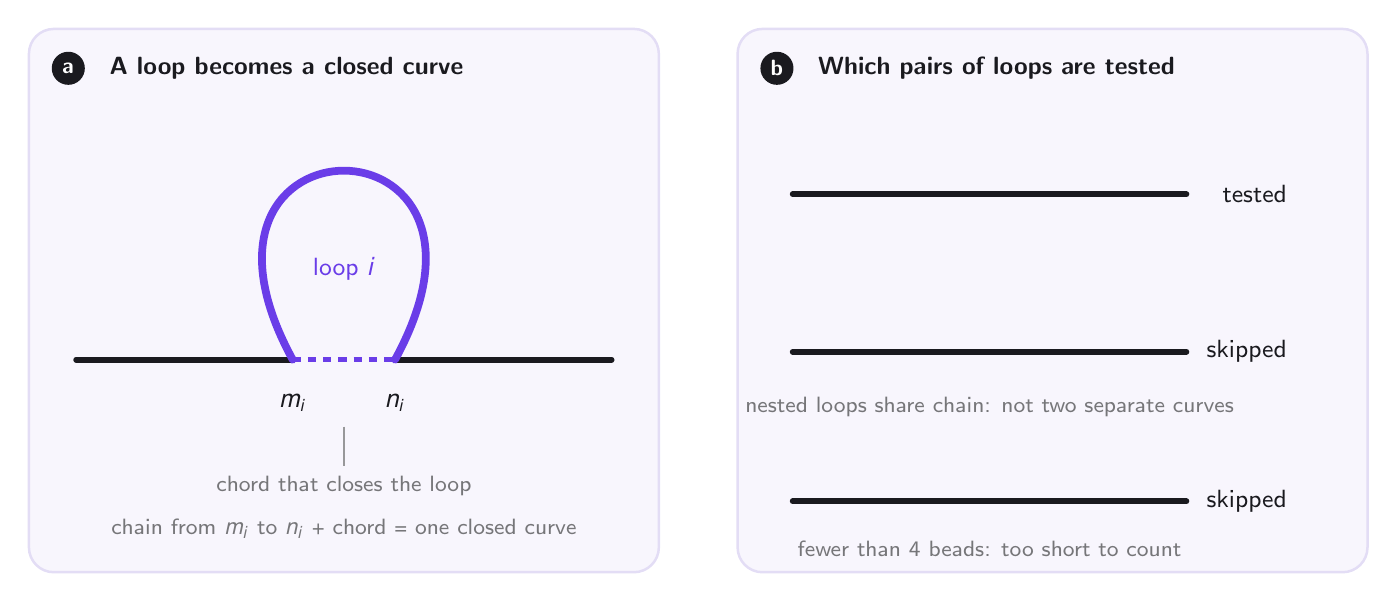
\begin{tikzpicture}
  \panelbg{0}{-3.3}{8}{3.6}\panelbg{9}{-3.3}{17}{3.6}
  \badge{0.5}{3.1}{a}\node[hd] at (0.9,3.1) {A loop becomes a closed curve};\badge{9.5}{3.1}{b}\node[hd] at (9.9,3.1) {Which pairs of loops are tested};
  % a: chain, loop between legs m_i and n_i, and the chord that closes it
  \draw[fiber] (0.6,-0.6)--(3.35,-0.6);\draw[fiber] (4.65,-0.6)--(7.4,-0.6);
  \draw[cohesin,line width=2.8pt,line cap=round] (3.35,-0.6) .. controls (1.6,2.6) and (6.4,2.6) .. (4.65,-0.6);
  \draw[cohesin,line width=1.6pt,dash pattern=on 3pt off 2.5pt] (3.35,-0.6)--(4.65,-0.6);
  \legdot{3.35}{-0.6}{cohesin}\legdot{4.65}{-0.6}{cohesin}
  \node[lab] at (3.35,-1.15) {$m_i$};\node[lab] at (4.65,-1.15) {$n_i$};
  \node[lab,cohesin] at (4,0.55) {loop $i$};
  \draw[leader] (4.0,-1.45)--(4.0,-1.95) node[note,below] {chord that closes the loop};
  \node[note,align=center] at (4,-2.75) {chain from $m_i$ to $n_i$ $+$ chord $=$ one closed curve};
  % b: three arrangements
  \begin{scope}[shift={(9.7,1.5)}]\draw[fiber] (0,0)--(5.0,0);\arcl{0.5}{2.1}{li}\arcl{3.0}{4.6}{lj}\legdot{0.5}{0}{cohesin}\legdot{2.1}{0}{cohesin}\legdot{3.0}{0}{ink}\legdot{4.6}{0}{ink}\end{scope}
  \node[lab,anchor=east] at (16.1,1.5) {tested};\ok{16.55}{1.5}
  \begin{scope}[shift={(9.7,-0.5)}]\draw[fiber] (0,0)--(5.0,0);\arcl{0.5}{4.6}{li}\arcl{1.6}{3.5}{lj}\legdot{0.5}{0}{cohesin}\legdot{4.6}{0}{cohesin}\legdot{1.6}{0}{ink}\legdot{3.5}{0}{ink}\end{scope}
  \node[lab,anchor=east] at (16.1,-0.5) {skipped};\no{16.55}{-0.5}
  \node[note,align=center] at (12.2,-1.2) {nested loops share chain: not two separate curves};
  \begin{scope}[shift={(9.7,-2.4)}]\draw[fiber] (0,0)--(5.0,0);\arcl{0.5}{1.0}{li}\arcl{3.0}{4.6}{lj}\legdot{0.5}{0}{cohesin}\legdot{1.0}{0}{cohesin}\legdot{3.0}{0}{ink}\legdot{4.6}{0}{ink}\end{scope}
  \node[lab,anchor=east] at (16.1,-2.4) {skipped};
  \node[note] at (12.2,-3.0) {fewer than 4 beads: too short to count};\no{16.55}{-2.4}
\end{tikzpicture}
\end{document}
